\section{Trenowanie}\label{sec:trenowanie}
\subsection{Sieć neuronowa}\label{subsec:trenowanie_siec_neuronowa}
\subsubsection{Architektura}\label{subsubsec:architektura_nn}
Sieć neuronowa składa się z warstw wejściowych, ukrytych i wyjściowych. Można ją przedstawić jako graf skierowany acykliczny.
Wagi połączeń między neuronami są losowane na początku i aktualizowane w trakcie uczenia.
\begin{figure}[H]
    \centering
    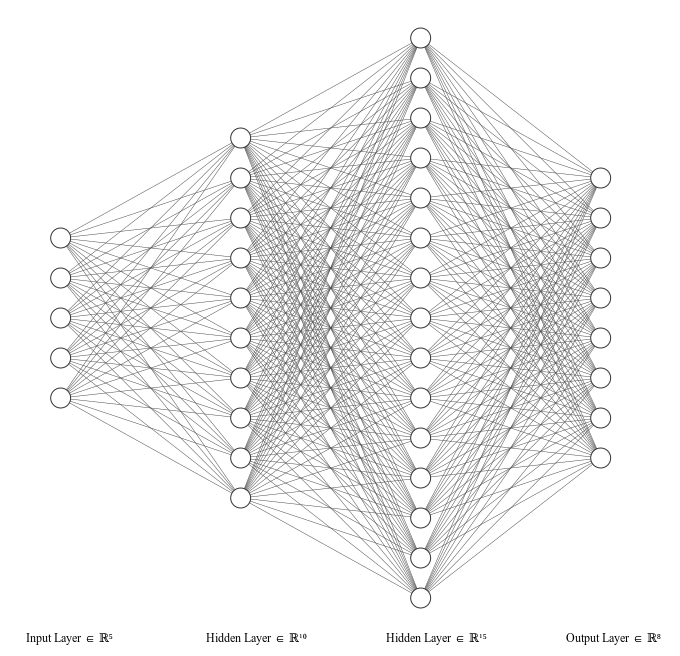
\includegraphics[width=0.6\textwidth]{img/nn.png}
    \caption{Poglądowy schemat sieci neuronowej.}
    \label{fig:neural_network}
\end{figure}
W tym badaniu ustalono optymalną architekturę sieci neuronowej na 4 warstwy:
\begin{itemize}
    \item warstwa wejściowa - 16 neuronów, po jednym na każdą cechę
    \item pierwsza warstwa ukryta - 128 neuronów
    \item druga warstwa ukryta - 256 neuronów
    \item warstwa wyjściowa - 26 neuronów, po jednym na każdą literę alfabetu angielskiego
\end{itemize}
\subsubsection{Funkcja aktywacji}\label{subsubsec:funkcja_aktywacji}
Funkcja aktywacji jest funkcją, która przekształca sumę ważoną wejść neuronu na jego wyjście.
Gdyby nie było funkcji aktywacji, to sieć neuronowa byłaby liniowa, a wtedy nie byłaby w stanie nauczyć się złożonych zależności.
W tym badaniu użyto funkcji ReLU na warstwach ukrytych (ang. \textit{Rectified Linear Unit}) oraz softmax na wyjściowej.
\begin{equation}
    f(x) = max(0, x)
\end{equation}
\begin{figure}[H]
    \centering
    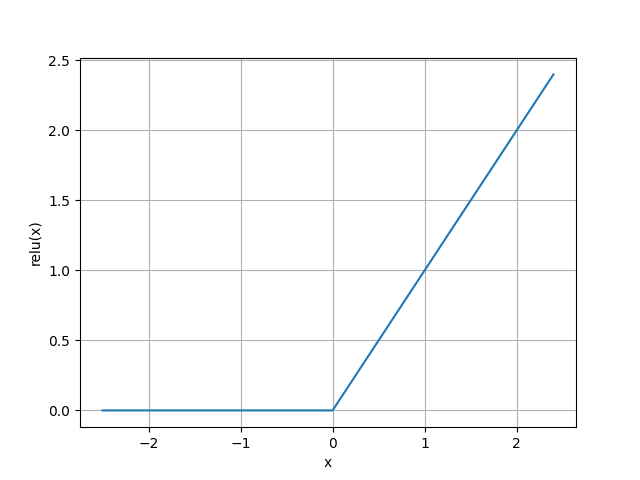
\includegraphics[width=0.6\textwidth]{img/relu.png}
    \caption{Funkcja ReLU.}
    \label{fig:relu}
\end{figure}
Funkcja softmax jest funkcją, która przekształca wektor liczb rzeczywistych na wektor liczb z przedziału [0, 1].
Suma wszystkich wartości wektora wyjściowego jest równa 1, więc można go interpretować jako rozkład prawdopodobieństwa.
W przypadku użycia jako funkcja aktywacji w warstwie wyjściowej, największa wartość wektora wyjściowego traktowana jest jako wynik klasyfikacji.
\begin{equation}
    \label{eq:softmax}
    f(x_i) = \frac{e^{x_i}}{\sum_{j=1}^{n} e^{x_j}}
\end{equation}
\subsubsection{Funkcja straty}\label{subsubsec:funkcja_straty}
Funkcja straty jest funkcją, która określa jak bardzo wynik klasyfikacji różni się od oczekiwanego.
Ze względu na to, że wyjście sieci neuronowe nie jest jako wektor one-hot
(wektor, w którym tylko jedna wartość jest równa 1, a reszta 0),
wykorzystano funkcję entropii krzyżowej kategorycznej (ang. \textit{sparse categorical cross-entropy}).
\begin{equation}
    f(y, \hat{y}) = -\sum_{i=1}^{n} y_i \log(\hat{y_i})
\end{equation}
Gdzie $y$ to wektor oczekiwanych wyjść, a $\hat{y}$ to wektor wyjść sieci neuronowej.
\subsubsection{Uczenie sieci}\label{subsubsec:uczenie_sieci}
Uczenie sieci neuronowej polega na aktualizacji wag połączeń między neuronami.
Najważniejszymi parametrami podczas trenowania sieci neuronowej są:
\begin{itemize}
    \item współczynnik uczenia (ang. \textit{learning rate}). Określa jak bardzo aktualizowane są wagi po każdej iteracji.
    \item funkcja optymalizująca (ang. \textit{optimizer}). Określa jak aktualizowane są wagi po każdej iteracji.
    \item funkcja straty (ang. \textit{loss function}). Określa jak bardzo wynik klasyfikacji różni się od oczekiwanego.
    \item liczba epok (ang. \textit{epochs}). Określa ile razy sieć neuronowa przejdzie przez cały zbiór danych.
\end{itemize}
W tym badaniu użyto następujących parametrów:
\begin{itemize}
    \item współczynnik uczenia - 0.001
    \item funkcja optymalizująca - Adam
    \item funkcja straty - entropia krzyżowa kategoryczna
    \item liczba epok - 40
\end{itemize}
\subsubsection{Czas trenowania}\label{subsubsec:czas_trenowania_nn}
Czas trenowania sieci neuronowej zależy od wielu czynników, takich jak:
\begin{itemize}
    \item liczba warstw
    \item liczba neuronów w warstwach
    \item liczba epok
    \item liczba danych
    \item złożoność danych
    \item parametry trenowania
    \item sprzęt
\end{itemize}
Jak wcześniej wspomniano, sieć jest relatywnie mała i prosta, dane niezbyt obszerne, ani złożone, a parametry trenowania nie są zbyt wymagające.
W związku z tym, czas trenowania sieci neuronowej nie jest długi, nawet na słabszym sprzęcie.
Do trenowania wykorzystano łatwo dostępny sprzęt, który nie jest dedykowany do uczenia maszynowego: procesor AMD Ryzen 5 5600 6-core 3.7GHz wraz z 32GB RAM.
Czas trenowania sieci neuronowej wyniósł około 15 sekund dla danych niezbalansowanych, 17 dla over sampled oraz około 13 dla under sampled.
\subsubsection{Dokładność i strata podczas treningu}\label{subsubsec:dokladnosc_i_strata_podczas_treningu}
Dokładność i strata podczas treningu są miarami określającymi jak dobrze sieć neuronowa radzi sobie z klasyfikacją na zbiorze walidacyjnym po każdej iteracji trenowania.
W idealnym świecie dokładność powinna rosnąć do 100\% dokładności, a strata maleć do 0. Jednak w rzeczywistości nie jest to możliwe, bądź nie jest to opłacalne.
Ryzykujemy bowiem przeuczeniem sieci neuronowej, co oznacza, że sieć będzie zbyt dobrze radzić sobie z danymi treningowymi, ale nie będzie w stanie dobrze klasyfikować nowych danych.
W trenowaniu sieci neuronowej zależy nam na generalizowaniu, czyli na tym, żeby sieć dobrze radziła sobie z różnymi danymi, a nie tylko tymi, na których była trenowana.
\begin{figure}[H]
    \begin{subfigure}{.33\textwidth}
        \centering
        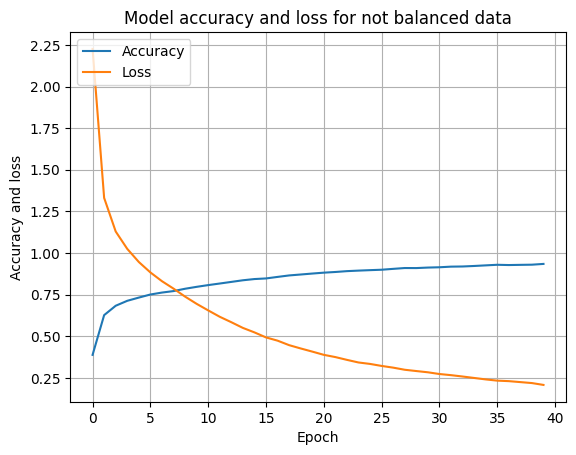
\includegraphics[width=\textwidth]{img/not_balanced_acc_loss.png}
        \caption{Niezbalansowane.}
        \label{fig:accu_loss_not_balanced}
    \end{subfigure}
    \begin{subfigure}{.33\textwidth}
        \centering
        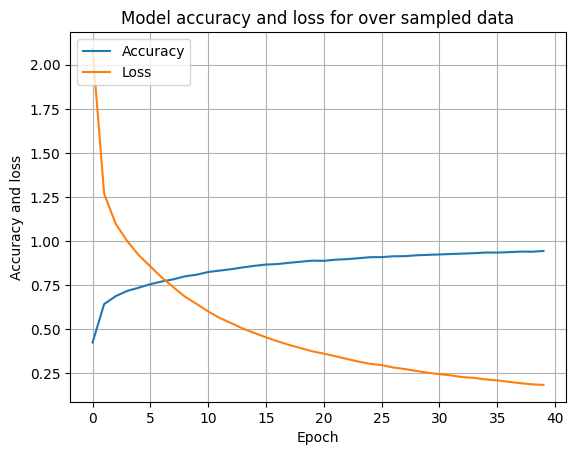
\includegraphics[width=\textwidth]{img/over_acc_loss.png}
        \caption{Over sampling.}
        \label{fig:loss}
    \end{subfigure}
    \begin{subfigure}{.33\textwidth}
        \centering
        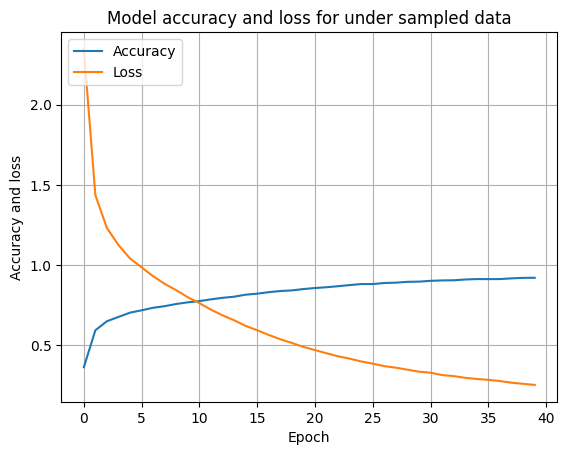
\includegraphics[width=\textwidth]{img/under_acc_loss.png}
        \caption{Under sampling.}
        \label{fig:accu_loss_under}
    \end{subfigure}
    \caption{Dokładność i strata podczas treningu względem liczby epok.}
\end{figure}
Widoczne jest duże podobieństwo między wykresami dokładności i straty dla wszystkich trzech przypadków.
Widoczne jest też poprawne zachowanie się sieci neuronowej: dokładność rośnie do 1, a strata maleje do 0.
\subsection{K najbliższych sąsiadów}\label{sec:k_najblizszych_sasiadow}
\subsubsection{Algorytm}\label{subsubsec:algorytm}
Algorytm k najbliższych sąsiadów (ang. \textit{k nearest neighbors}) jest algorytmem uczenia maszynowego, który klasyfikuje dane na podstawie ich najbliższych sąsiadów.
W przeciwieństwie do sieci neuronowej, algorytm k najbliższych sąsiadów nie uczy się na podstawie danych, tylko przechowuje je w pamięci.
Klasyfikacji dokonuje się poprzez znalezienie k najbliższych sąsiadów i wybraniu najczęściej występującej klasy.
\begin{figure}[H]
    \centering
    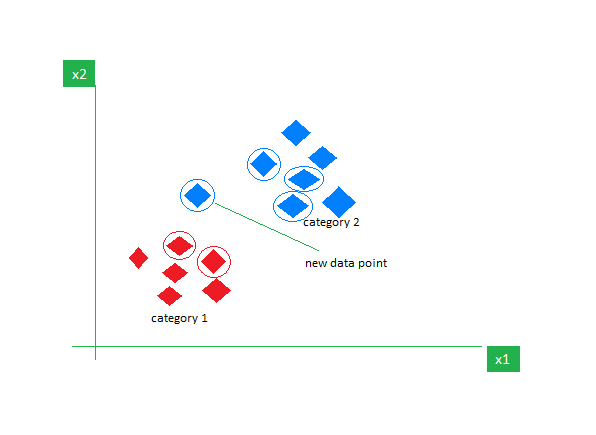
\includegraphics[width=0.8\textwidth]{img/knn.png}
    \caption{Poglądowy schemat algorytmu k najbliższych sąsiadów.}
    \cite{knn-GeeksforGeeks_2023} 
    \label{fig:knn}
\end{figure}
\subsubsection{Parametry}\label{subsubsec:parametry}
Parametrami algorytmu k najbliższych sąsiadów są:
\begin{itemize}
    \item liczba sąsiadów (ang. \textit{n\_neighbors}). Określa ile najbliższych sąsiadów zostanie wybranych.
    \item metryka (ang. \textit{metric}). Określa jak będzie liczona odległość między danymi.
\end{itemize}
W tym badaniu użyto następujących parametrów:
\begin{itemize}
    \item liczba sąsiadów - 3
    \item metryka - euklidesowa
\end{itemize}
\subsubsection{Czas trenowania, dokładność i strata}\label{subsubsec:czas_trenowania_knn}
Tak jak wcześniej wspomniano, algorytm k najbliższych sąsiadów tylko przechowuje w pamięci dane treningowe, a co za tym idzie, nie wymaga trenowania - czas jest równy 0 
(pomijając elementy czysto sprzętowo-techniczne jak odczytanie i załadowanie danych do pamięci).
Z tego też powodu dokładność i strata nie są miarami, które można określić dla algorytmu k najbliższych sąsiadów.
